\chapter{Diseño}

\section{Enfoque del proyecto}
\subsection{Proyecto como aplicación final}
Como punto de partida inicial se plantea el desarrollo de una aplicación completa y autosuficiente, para su instalación en un dispositivo móvil Android.

Como ventajas de este enfoque el usuario no depende de la disponibilidad del servidor donde se aloja la aplicación, ya que la ésta se instala en su propio dispositivo, además al operar localmente suelen ofrecer un menor tiempo de respuesta. Sin embargo, también presenta desventajas, como el mayor esfuerzo para actualizar la aplicación en cada dispositivo, ya que recae en el usuario o la limitación del entorno, que dificulta la flexibilidad y escalabilidad, integrar nuevas funcionalidades o realizar cambios son tareas más complejas de realizar porque afectan a todo el proyecto.

\subsection{Proyecto como servicio}
Un proyecto como servicio es una aplicación modular y distribuida en la que el backend funciona como un servicio independiente de la plataforma, permitiendo la interacción con varios tipos de clientes (web, móvil, etc.) con conexión a Internet. 

Presenta gran flexibilidad ante la impementación de mejoras, ya que se pueden realizar cambios en el backend sin afectar al frontend, y viceversa. Como puede ser agregar nuevas funcionalidades o módulos (como más servicios de análisis de gastos o incorporar diferentes funcionalidades de ahorro) sin afectar el resto del sistema. A medida que los usuarios crecen, el backend como servicio puede escalarse fácilmente. De esta manera, se adapta bien a un entorno donde puede servir como base para otros clientes o dispositivos, es un sistema más versátil y eficiente. Sin embargo, también presenta desventajas, como dependencia de la red, ya que requiere una conexión estable entre cliente y servidor, lo cual puede ser una limitación si el servicio se utiliza sin darse esa condición. Implementar un proyecto como servicio suele requerir un esfuerzo inicial mayor que la aplicación final para planificar y configurar una arquitectura escalable y segura\cite{galster2014variability}.\\


Dadas las dos opciones anteriores, la que mejor se adapta a este proyecto es el enfoque como servicio, ya que se espera que la aplicación pueda ser utilizada por un número creciente de usuarios y que se puedan implementar mejoras frecuentes y nuevas funcionalidades en el futuro, motivado principalmente por el uso de metodología ágil en el desarollo de la misma. Además permite el acceso multiplataforma, aunque se considera útil la aplicación para dispositivos móviles, no se quiere limitar el alcance de la misma, sino también poder consultar el conjunto de movimientos desde ordenadores, que nos ofrecen mayor comodidad para analizar los datos. De este modo se va a priorizar como aproximación inicial una solución que se pueda usar como mínimo desde cualquiera de estos dos tipos de dispositivos. Se opta por una aplicación web, donde el backend funciona como un servicio independiente y el frontend como cliente.

\begin{figure}[ht!]
    \centering
    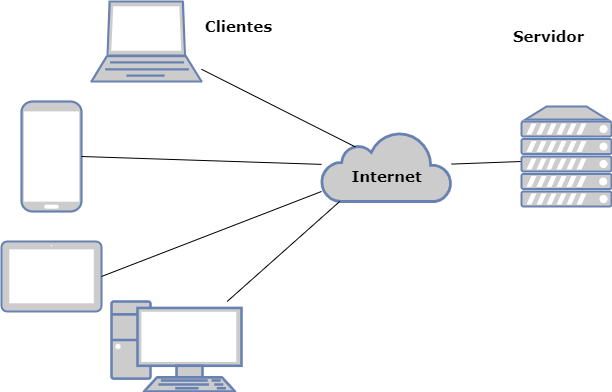
\includegraphics[height = 50mm]{imagenes/proyecto_servicio.drawio.png}
    \caption{Proyecto como servicio}
    \label{fig:proyecto_como_servicio}
    \end{figure}


\section{Arquitectura software}
Para definir la arquitectura de software de la aplicación, se analizaron varias opciones disponibles, cada una con características y beneficios diferentes\cite{albin2003art}\cite{garimilla2024art}:

\begin{itemize}
\item Arquitectura Monolítica\\
Las arquitecturas monolíticas agrupan todos los componentes de la aplicación en una única unidad de despliegue, lo cual facilita la implementación y es adecuado para aplicaciones pequeñas o medianas. Sin embargo, este enfoque suele presentar limitaciones en cuanto a flexibilidad y escalabilidad, ya que todos los módulos están estrechamente acoplados. Lo que provoca que las opciones de actualización y expansión se vean reducidas.

\item Arquitectura Basada en Microservicios\\
Una arquitectura de microservicios organiza la aplicación en servicios pequeños e independientes que pueden desarrollarse, desplegarse y escalarse de manera autónoma. Cada microservicio puede implementarse con el lenguaje y las herramientas más adecuadas para su función, lo que aporta flexibilidad y facilita la escalabilidad. Además, su naturaleza distribuida añade seguridad, ya que los servicios se comunican a través de una API y no de manera directa, ofreciendo una capa adicional de protección. Sin embargo, esta estructura aumenta la complejidad de implementación y requiere mayor infraestructura, lo cual puede ser innecesario para aplicaciones con un alcance más específico\cite{RedHat2023}\cite{lopez2017arquitectura}.

\item Arquitectura Cliente-Servidor\\
La arquitectura cliente-servidor divide la aplicación en dos componentes principales: el cliente (interfaz de usuario) y el servidor (lógica de negocio y acceso a datos). La comunicación entre cliente y servidor se puede gestionar mediante una API REST (Representational State Transfer), que utiliza solicitudes HTTP \footnote{HyperText Transfer Protocol: es un protocolo cliente-servidor para comunicar aplicaciones por medio de peticiones de datos y recursos} (como GET, POST, PUT y DELETE) para intercambiar información. Este enfoque proporciona una separación clara entre la interfaz y la lógica de negocio, facilitando el mantenimiento y la escalabilidad sin necesidad de una infraestructura compleja como en el caso de los microservicios.

\end{itemize}

Los enfoques tradicionales con arquitectura monolítica limitan a los desarrolladores en cuanto al lenguaje de programación y entorno de ejecución. Por otro lado, las otras dos opciones permiten a los desarrolladores elegir el lenguaje de programación y el entorno de ejecución más adecuado para cada servicio. Además, por su naturaleza distribuida facilitan la escalabilidad y la flexibilidad del sistema, y aportan seguridad al actuar como una primera línea de defensa ante ataques, ya que los servicios se comunican entre sí por ejemplo mediante una API y no directamente. 

La arquitectura basada en microservicios no se justifica para las necesidades actuales del proyecto, que al resolver una necesidad específica no se beneficia de las ventajas que ofrece pero si podría verse afectado su desarrollo por la complejidad que añade. 

En su lugar, se ha optado por implementar una arquitectura cliente-servidor para la aplicación, donde el cliente (generalmente un navegador web) se corresponde con la interfaz de usuario y el servidor gestiona la lógica de negocio y la base de datos. La comunicación entre ambos se realiza mediante una API REST. Esto permite modularidad, escalabilidad, y facilidad de mantenimiento, facilitando una futura migración a microservicios si es necesario, ya que la API REST puede servir como interfaz entre servicios independientes. La API REST en esta arquitectura conecta de forma sencilla y eficiente los datos y funcionalidades del backend con el frontend, pensada como una colección de herramientas escalable e independiente que realizan tareas específicas. 

\section{Herramientas de desarrollo}

\section{Diseño lógico}
Diagramas UML?

\section{Diseño wireframes / mockups / prototipos para el frontend}